\section{Response Time}
Response time is another major feature exploited in Internet traffic analysis attack. Again we would expect the same attacks can be applied to 6LoWPAN traffic and works even better than their counterparts against Internet traffic, as the accuracy of timing measurements can be greatly improved for 6LoWPAN traffic. 

Firstly, the devices are physically close to each other and uses RF to communicate. The adversary can remove the RTT noises by measure the packets on the server side. 

Secondly, performance of the constrained devices are low; hence gives a better resolution on timing code execution.

\subsection{Different Sensors}
%Plaintext recovery.
%\begin{itemize}
%	\item Reading different sensors takes different time.
%	\item Requirement: needs to identify CoAPS packets.
%	\item Works on both 802.15.4 Seuciryt and DTLS, if the requirement is met. 
%\end{itemize}

CoAP\cite{rfc7252} is a protocol designed for constraied devices that provides an universal interface for accessing resources. CoAPs is the secure version which stands for CoAP with DTLS.

Due to the different physical characters of sensors, there could be a variance of time when reading the measurements. The idea is to investigate whether such variance can be observed through the packet response latency.

We implemented the experiment on CC2538, using all three sensors from ``cc2538-demo", namely Vdd, temperature and Ambient Light Sensor (ALS). We used CoAP from the ``er-rest-example" in the Contiki OS source code, as there is no CoAPs implementation available. 

Although DTLS processing would definitely have an impact on the response latency, we argue that such impact would be independent to the sensors being accessed; hence similar result would hold even in case of CoAPs.

We have carefully crafted other factors, including URIs, data representation and code flow, to be uniform for all three sensors in order to guarantee a controlled environment.

\begin{table}
	\center
	\begin{tabular}{|c|c|c|}
	\hline
	& Average (ms) & Range(ms) \\ 
	\hline
	Vdd & 9.622 & [9.388, 10.318] \\ 
	\hline
	Temperature & 9.835 & [9.525, 10.318] \\ 
	\hline
	ALS & 11.651 & [11.338, 12.031] \\
	\hline
\end{tabular} 
	\caption{CoAP Response Latency for Sensor Readings on CC2538\label{CoapTiming}}
\end{table}

\Cref{CoapTiming} summarises the result. It is shown that ALS takes about $2$ms longer and hence can be easily distinguished. Vdd and temperature might be difficult to distinguish by response latency as they have similar results.



\subsection{Different Hardware}
%Gain hardware information.
%\begin{itemize}
%	\item Different hardware has different response latency against the same message.
%	\item For 802.15.4: Requires additional information. Can be satisfied by the previous ICMP attack.
%	\item For DTLS: No requirement. The adversary can actively send a message, e.g. PING.
%\end{itemize}

A more general leakage is the response latency to a specific message, as different processors would have different computational power and thus different time to process a same message. The ICMP messages turns out to be suitable for this attack since they are standardised and thus universally supported. Among the ICMP messages, PING is especially ideal for two reasons: 
\begin{enumerate}
	\item It is mandatory in the ICMP standard.
	\item It only swaps the source and destination address of the packet; thus minimises different code path in protocol processing.
\end{enumerate}

\begin{table}
	\center
	\begin{tabular}{|c|c|c|}
	\hline
			& CC2538	& TelosB \\ 
	\hline
	Average(ms)	& 9.56		& 17.03 \\ 
	\hline
	Range(ms)	& [9.16, 10.06]	& [16.49, 17.68]	\\
	\hline
\end{tabular}

	\caption{PING Response Latency\label{PingResponse}}
\end{table}

\Cref{PingResponse} shows the PING response latency on CC2538 and TelosB. The result confirms that these devices can be distinguished by PING response latency.

\subsection{Program Fingerprint}
%Fingerprints the code running on a device, which leads to plaintext recovery.
%\begin{itemize}
%	\item Theory explained in \Cref{FingerprintTheory}.
%	\item Requirement: needs to actively send messages. Any Request/Response protocol works, such as PING, DTLS Heartbeat, CoAP PING, etc. 
%	\item Not for 802.15.4: adversary can't join the network.
%	\item For DTLS: PING is available and confirmed. DTLS Heartbeat should work if supported.
%\end{itemize}
The response time of packets could also be exploited to fingerprint the code running on a specific device. 

\subsubsection{Hypothesis}
%How it works
\Cref{FingerprintTheory} illustrates two sensors receiving a same service request. Sensor Node 1 was idle and hence responded immediately, whilst Sensor Node 2 postponed the request for reading a sensor. From the aspect of packets, the response time on Sensor Node 2 would appear longer than that of Sensor Node 1.

\begin{figure}
	\center
	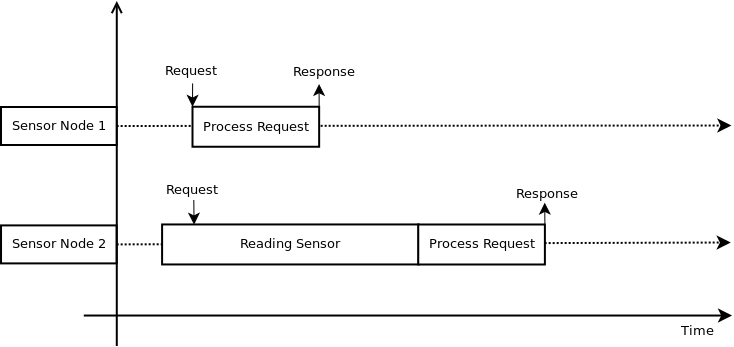
\includegraphics[width=\textwidth]{fig/PingProbe_Theory.png}
	\caption{Variations in Response Time\label{FingerprintTheory}}
\end{figure}

Most sensors are programmed in a loop; therefore the same code fragments are repeated through the life time of a sensor. Each code fragment takes different time to execute and hence extends response time differently. 

The code fingerprinting attack exploits this phenomenon by statically analysing the distribution of extended response time to reveal information of the program.

\begin{definition}
	We refer the distribution of extended response time as a \textbf{``fingerprint''} to the program running on the sensor node.
\end{definition}

For this attack, we assume the adversary has the pre-knowledge of potential programs, together with a database of all their fingerprints. To identify an unknown program running on target sensor, the adversary collects its fingerprint and then matches it to the database.

To effectively launch the attack, the adversary also needs to be able to send the requests. Further more, requests with short predictable processing time are preferable as they induce less noise. 

In practice, the request can be instantiated by several messages defined in the sensor network protocols. PING is exceptionally ideal as it is mandatory in the ICMP standard\cite{rfc4433} and has only negligible computation. Other options but not excluded are Heartbeat in DTLS\cite{rfc6520}, Reset in CoAP\cite{rfc7252}, etc.

\subsubsection{Extracting Fingerprint}
The first task of the attack is to construct a fingerprint of a program. We experimented with PING on CC2538 running Contiki OS. 

\Cref{ExamplePri} shows an example of captured packets. Contiki MAC\cite{ContikiMAC} sends duplicated PING requests. The response time, refers to PING Response Interval, PRI, is defined to be the time between a PING response and its last paired request. The highlighted Packet 205 and Packet 203 shows such an example.

\begin{figure}[!h]
	\centering
	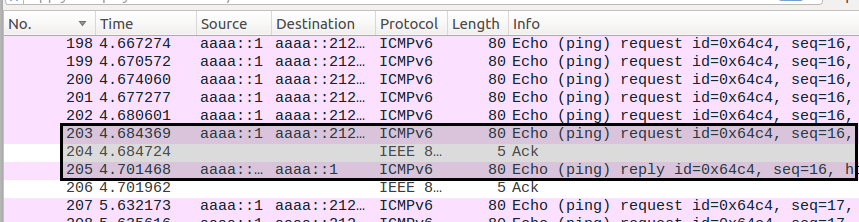
\includegraphics[width=\textwidth]{fig/PRI_hl.png}
	\caption{Example PRI\label{ExamplePri}}
\end{figure}

%Since the attack extracts the information contained in the extended response time of a specific request, the first problem is to see whether such extended response time can be filtered from normal ones. 

\Cref{HelloworldPriNormal} shows the histogram of PRIs collected on the ``helloworld'' example from Contiki OS. Values $\geq$12ms are collected at 12ms. The result shows that most PRIs are clustered around 9.5ms which consists with our result in \Cref{PingResponse}. The majority, roughly ranged [9.0, 10.3]ms, corresponds to the usual response time as depicted by Sensor Node 1 in \Cref{FingerprintTheory}. 

\begin{figure}[!h]
	\centering
	\begin{subfigure}{0.45\textwidth}
		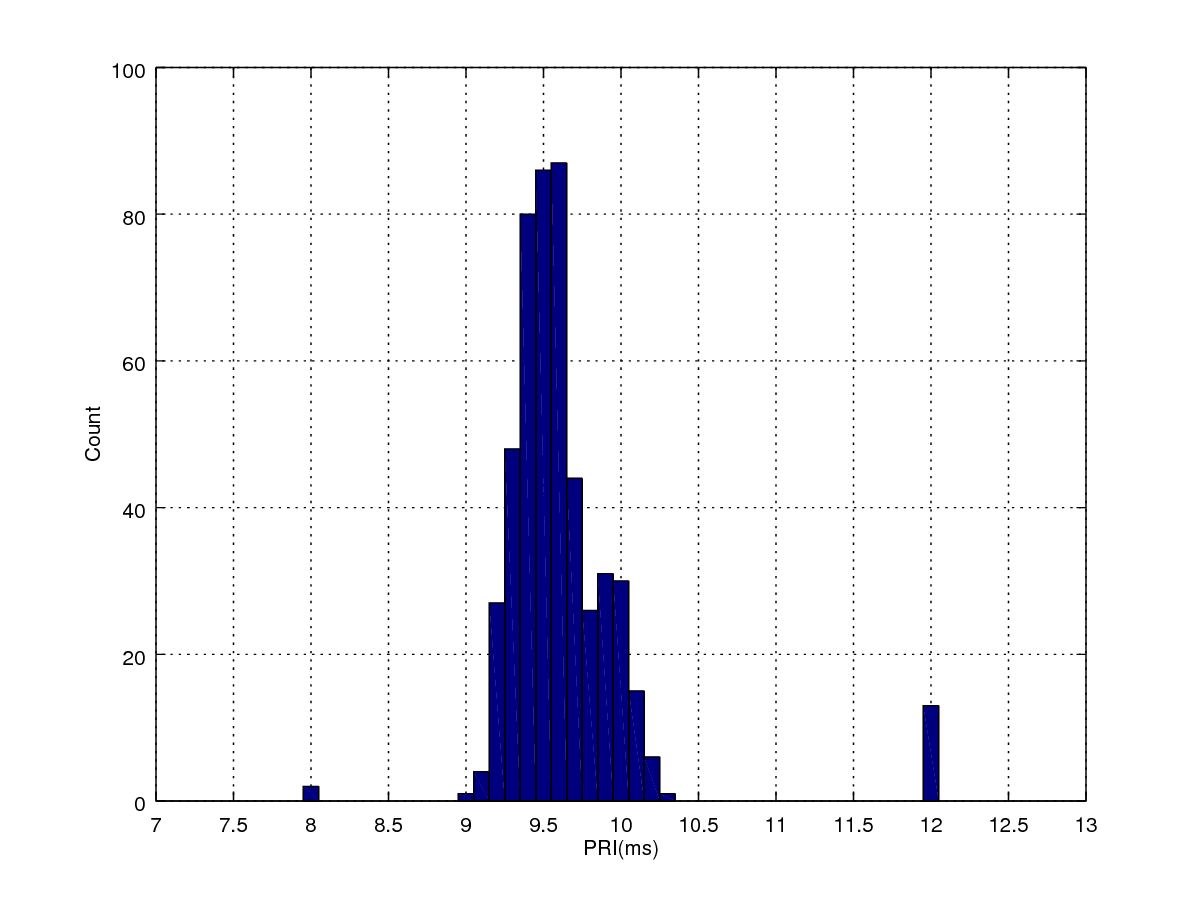
\includegraphics[width=\textwidth]{fig/helloworld_cc2538.png}
		\caption{PRIs of helloworld\label{HelloworldPriNormal}}
	\end{subfigure}
	\begin{subfigure}{0.45\textwidth}
		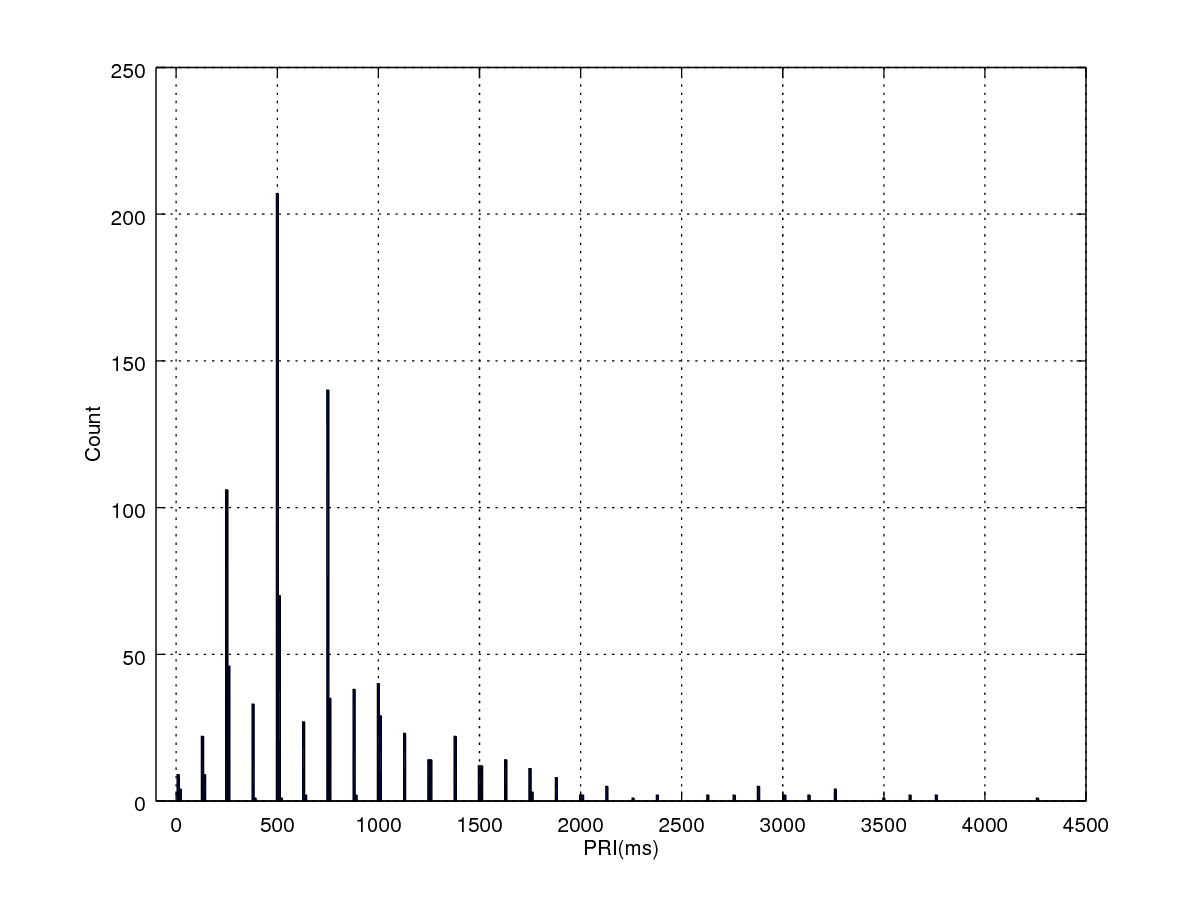
\includegraphics[width=\textwidth]{fig/helloworld_cc2538_outlier.png}
		\caption{PRIs outliers of helloworld\label{HelloworldPriOutliers}}
	\end{subfigure}
	\caption{helloworld PRIs\label{HelloworldPri}}
\end{figure}

We further plotted the upper outliers, mostly ranged [12, 2000]ms, in \Cref{HelloworldPriOutliers}. We suppose these outliers corresponds to the extended response time as depicted by Sensor Node 2 in \Cref{FingerprintTheory}. According to the hypothesis, the distribution described by \Cref{HelloworldPriOutliers} is the fingerprint of the ``helloworld'' example.

The result in \Cref{HelloworldPri} showed a clear gap between the usual PRIs and extended PRIs. In fact other applications we experimented also showed the same property. This implies that an adversary can easily draw a threshold by observing the whole PRI distribution and then filters the fingerprint. In our experiments the threshold is set to 12ms but any other values within the gap would also work. 

\subsubsection{Fingerprint Matching}
%Comparing the distribution.
We collected the fingerprints for three programs taken from the Contiki OS examples:
\begin{description}
	\item[broadcast] This is taken as it is from the example which periodically broadcasts a constant message.
	 
	\item[powertrace] This is taken as it is from the example which records the power consumption and broadcasts a constant message.
	
	\item[Sensorpayload] This program is based on the ``er-rest-example'' embedded together with sensor accesses taken from ``cc2538-demo''. It captures a real case scenario where three different sensors, namely Temperature, VDD and ALS, are being access through CoAP.
\end{description}

Specifically for ``Sensorpayload'' we collected fingerprints for 8 different scenarios where different sensors are being accessed. For each program we independently collected 2 fingerprints for comparison.

\Cref{FingerprintApps} summarises the total 20 fingerprints we collected for the experiment.

During the experiments we realised that most of the fingerprints does not subject to any common distributions as expected; therefore we used Kolmogorov-Smirnov Distance as the statistics. \Cref{ksdistances} summarises the relative KS distances computed on each pair of fingerprints in our experiments.

Although fingerprints collected on the same application basically failed to pass the Kolmogorov-Smirnov Test, we realised that their KS distance tends to be smaller comparing to fingerprints collected on different programs, as the \textbf{bold} cells marked in \Cref{ksdistances}. 

By matching fingerprints with the minimum KS distance, 13 out of 20 fingerprints in our experiments have successfully matched the paired one collected on the same program, which suggests a much better result than random matching.

Further more the mismatch only occur among the ``Sensorpayload'' program and fingerprints collected on the same program still tends to have relatively low KS distances. Considering they share most of the code except a slight difference in reading different sensors, the KS distances of fingerprints might also be suggested as a support measurement of similarity of different programs.

\subsection{Countermeasure}
%Two options:
%\begin{itemize}
%	\item Randomise response time: needs to be resilient to statistical analysis.
%	\item Threashold response time (discard or reply in a constant time): performance tradeoff. Recommended for unreliable transmissions.
%\end{itemize}
Timing countermeasures are relatively hard to be implemented due to hardware restrictions. There are two common countermeasures considered:
\begin{itemize}
	\item Randomly delay the response. However, the randomness must be carefully chosen to be statistically resilient which indicates potential computational overhead.
	 
	\item Use threshold response time, i.e. a request is either responded at a predefined time or not responded at all. This method is recommended as most 6LoWPAN application would tolerate missing packets and timer is available on most platforms. However, the threshold must be carefully chosen to preserve the functionality of the 6LoWPAN application.
\end{itemize}